\documentclass[12pt,border=3mm]{standalone}
\usepackage[T1]{fontenc}
\usepackage{lmodern,amsmath,amssymb,tikz}
\usetikzlibrary{arrows.meta,positioning,calc}
\definecolor{plantblue}{HTML}{247BA0}
\definecolor{plantteal}{HTML}{16856B}
\definecolor{plantorange}{HTML}{D97425}
\definecolor{plantpurple}{HTML}{7954A1}
\begin{document}
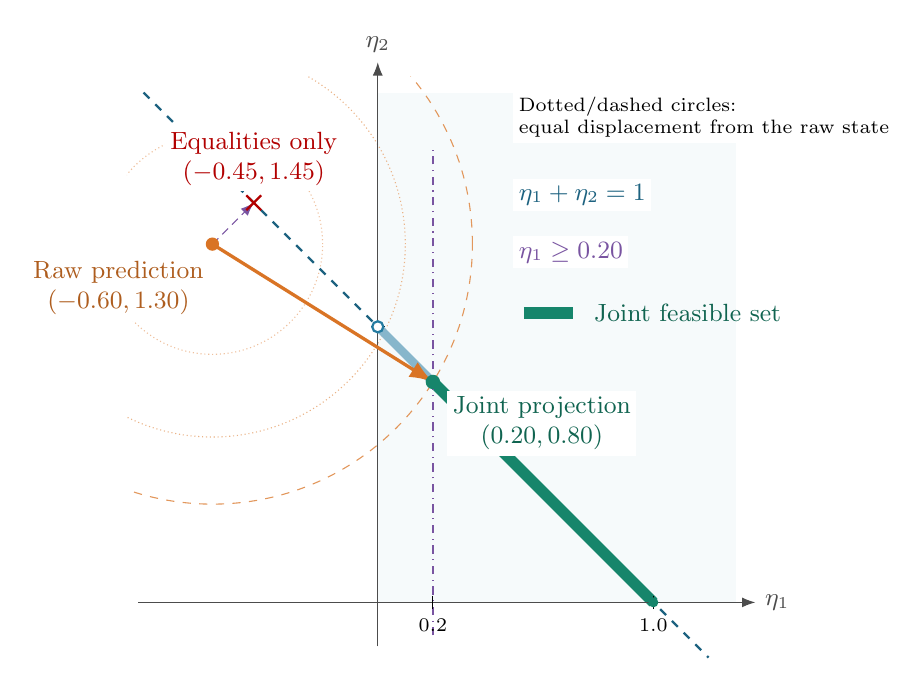
\begin{tikzpicture}[>=Latex,x=3.5cm,y=3.5cm,font=\small,
annotation/.style={fill=white,inner sep=2pt,align=center,font=\small}]
\fill[plantblue!4] (0,0) rectangle (1.30,1.85);
\begin{scope}
\clip (-.91,-.22) rectangle (1.31,1.91);
\draw[plantorange!45,densely dotted] (-.60,1.30) circle (.40);
\draw[plantorange!55,densely dotted] (-.60,1.30) circle (.70);
\draw[plantorange!75,dashed] (-.60,1.30) circle (.9433981);
\draw[plantblue!80!black,dashed,thick] (-.85,1.85)--(1.20,-.20);
\end{scope}
\draw[plantblue!55,line width=3pt] (0,1)--(1,0);
\draw[plantteal,line width=4pt] (.20,.80)--(1,0);
\draw[plantpurple,dash dot,thick] (.20,-.12)--(.20,1.65);
\draw[->,black!70] (-.87,0)--(1.37,0) node[right] {$\eta_1$};
\draw[->,black!70] (0,-.16)--(0,1.96) node[above] {$\eta_2$};
\foreach \tick in {0.2,1.0}{\draw (\tick,.025)--(\tick,-.025) node[below,font=\scriptsize] {$\tick$};}
\draw (.025,1)--(-.025,1);
\draw[plantorange,->,line width=1.2pt] (-.60,1.30)--(.20,.80);
\draw[plantpurple,->,densely dashed] (-.60,1.30)--(-.45,1.45);
\fill[plantorange] (-.60,1.30) circle (2.4pt);
\node[annotation,anchor=north east,text=plantorange!80!black] at (-.61,1.26) {Raw prediction\\$(-0.60,1.30)$};
\draw[red!70!black,thick] (-.477,1.423)--(-.423,1.477);
\draw[red!70!black,thick] (-.477,1.477)--(-.423,1.423);
\node[annotation,anchor=south,text=red!70!black] at (-.45,1.49) {Equalities only\\$(-0.45,1.45)$};
\draw[plantblue,fill=white,thick] (0,1) circle (2.0pt);
\fill[plantteal] (.20,.80) circle (2.6pt);
\node[annotation,anchor=north west,text=plantteal!75!black] at (.25,.77) {Joint projection\\$(0.20,0.80)$};
\fill[plantteal] (1,0) circle (1.8pt);
\node[annotation,anchor=west,text=plantblue!80!black] at (.49,1.48) {$\eta_1+\eta_2=1$};
\node[annotation,anchor=west,text=plantpurple] at (.49,1.27) {$\eta_1\ge0.20$};
\draw[plantteal,line width=4pt] (.53,1.05)--(.71,1.05);
\node[font=\small,anchor=west,text=plantteal!75!black] at (.75,1.05) {Joint feasible set};
\node[annotation,anchor=west,font=\scriptsize,align=left] at (.49,1.76) {Dotted/dashed circles:\\equal displacement from the raw state};
\end{tikzpicture}
\end{document}
